% -*- coding: utf-8 -*-
\errorcontextlines=200
\documentclass[11pt,dvipdfmx,b5paper]{book}

\usepackage{times}
\usepackage{courier}
\usepackage{comment}
\usepackage{subfig}
\usepackage{graphicx}

\usepackage{enumitem}
\usepackage{url}
\usepackage{listings}
\usepackage{tikz} % Drawing sliding-tile
\usepackage{xcolor}

%%%%%%%%%%%%%%%%%%%%%
% Math
\usepackage{amsmath}
\usepackage{amsthm}
\usepackage{amssymb}
\usepackage{mathtools}
\DeclarePairedDelimiter\ceil{\lceil}{\rceil}
\DeclarePairedDelimiter\floor{\lfloor}{\rfloor}

%%%%%%%%%%%%%%%%%%%%%
% Format
\usepackage[Bjornstrup]{fncychap}
\usepackage{titlesec}
\usepackage[framemethod=TikZ]{mdframed}
\usepackage{booktabs}

\setcounter{secnumdepth}{3}
\renewcommand{\baselinestretch}{1.15}

\usepackage{appendix}
\usepackage{hyperref}
\usepackage{makeidx}
\makeindex


%%%%%%%%%%%%%%%%%%%%
% Algorithm
\usepackage[boxruled,linesnumbered,noend]{algorithm2e}
\SetKwInOut{Input}{Input}
\SetKwInOut{Output}{Output}
\SetKwInOut{Side}{Side effect}
\SetKwComment{Comment}{$\triangleright$}{}

\begin{document}


% \begin{figure}
%   \begin{tikzpicture}[scale=0.5]
%     % MDP i
\node [draw, circle, minimum size=0.7cm] (a) at (2, 2) {$a$};
\node [draw, circle, minimum size=0.7cm] (b) at (4, 2) {$b$};
\node [draw, circle, minimum size=0.7cm] (c) at (0, 4) {$c$};
\node [draw, circle, minimum size=0.7cm] (d) at (0, 2) {$d$};
\node [draw, circle, minimum size=0.7cm] (e) at (2, 0) {$e$};
\node [draw, circle, minimum size=0.7cm] (f) at (4, 0) {$f$};
\node [draw, circle, minimum size=0.7cm] (g) at (0, 0) {$g$};
\node [draw, circle, minimum size=0.5cm] at (0, 0) {};

\coordinate[above of=a] (init);

\draw[->] (init) -- (a);
\draw[-] (a) -- (b);
\draw[-] (a) -- (c);
\draw[-] (a) -- (d);
\draw[-] (b) -- (e);
\draw[-] (b) -- (f);
\draw[-] (c) -- (d);
\draw[-] (d) -- (g);
\draw[-] (e) -- (f);
\draw[-] (d) -- (g);

%   \end{tikzpicture}
% \end{figure}
% 
% \begin{figure}
%   \begin{tikzpicture}[scale=0.5]
%     % MDP i
\node (a0) at (4, 6) {$a$};

\node (b1) at (2, 4) {$b$};
\node (c1) at (4, 4) {$c$};
\node (d1) at (6, 4) {$d$};

\node (e2) at (0, 2) {$e$};
\node (f2) at (2, 2) {$f$};
\node (d2) at (4, 2) {$d$};
\node (c2) at (6, 2) {$c$};
\node (g2) at (8, 2) {$g$};

\node (f3) at (0, 0) {$f$};
\node (e3) at (2, 0) {$e$};
\node (a31) at (3, 0) {$a$};
\node (c3) at (4, 0) {$c$};
\node (g3) at (5, 0) {$g$};
\node (a32) at (6, 0) {$a$};

\draw[-] (a0) -- (b1);
\draw[-] (a0) -- (c1);
\draw[-] (a0) -- (d1);
\draw[-] (b1) -- (e2);
\draw[-] (b1) -- (f2);
\draw[-] (c1) -- (d2);
\draw[-] (d1) -- (g2);
\draw[-] (d1) -- (c2);
\draw[-] (e2) -- (f3);
\draw[-] (f2) -- (e3);
\draw[-] (d2) -- (a31);
\draw[-] (d2) -- (c3);
\draw[-] (d2) -- (g3);
\draw[-] (c2) -- (a32);

%   \end{tikzpicture}
% \end{figure}

% \begin{figure}
%   \begin{tikzpicture}[scale=0.5]
%     % Grid pathfinding

\foreach \x in {0,...,3}
  \foreach \y in {0,...,3}
    {\node [draw, circle, fill=black] (\x\y) at (1.5*\x, 1.5*\y) {};}

\foreach \x in {0,...,3}
  \foreach \y in {0,...,2}
           {\draw (1.5 * \x, 1.5 * \y) -- (1.5 * \x, 1.5 * \y + 1.5);}

\foreach \y in {0,...,3}
  \foreach \x in {0,...,2}
           {\draw (1.5 * \x, 1.5 * \y) -- (1.5 * \x + 1.5, 1.5 * \y);}
           
\foreach \x in {0,...,3}
         {\node at (1.5 * \x, -1) {\x};
          \node at (-1, 1.5 * \x) {\x};
         }

%   \end{tikzpicture}
% \end{figure}

% \begin{figure}
%   \begin{tikzpicture}[scale=0.5]
%     % Sliding tile puzzle

\draw (0, 0) grid (4, 4);

\foreach \x in {0,...,3}
  \foreach \y in {0,...,3}
  {
        \pgfmathsetmacro{\val}{int(\x+3*\y+1)}
        \ifthenelse{\x=3 \AND \y=3}{;}{
          \node at (\x + 0.5, 3 - \y + 0.5) {\val};
        }
  }

\draw[fill=gray] (3,0) rectangle (4, 1);

%   \end{tikzpicture}
% \end{figure}

% \begin{figure}
%   \texttt{Sequence1 -TCA----\\
Sequence2 ATCACG--\\
Sequence3 ATGAGG--\\
Sequence4 ---AGGCA

}
% \end{figure}

% \begin{figure}
%   \begin{tikzpicture}[scale=0.5]
%     \foreach \x in {0, 8}
  {
    \pgfmathsetmacro{\noise}{0.15}           
\node[draw,circle,fill=black] (1\x) at (\x+0, 0) {};
\node[draw,circle,fill=black] (2\x) at (\x+2, 1-\noise) {};
\node[draw,circle,fill=black] (3\x) at (\x+3+2*\noise, 2) {};
\node[draw,circle,fill=black] (4\x) at (\x+2-\noise, 3-\noise) {};
\node[draw,circle,fill=black] (5\x) at (\x+1, 2-2*\noise) {};
\node[draw,circle,fill=black] (6\x) at (\x+0, 3+\noise) {};
\node[draw,circle,fill=black] (7\x) at (\x-1+\noise, 1) {};
}

\foreach \a in {1,...,6}
  {
    \pgfmathsetmacro{\n}{int(\a+1)}
    \draw[-] (\a8) -- (\n8);
  }

\draw[-] (78) -- (18);

%   \end{tikzpicture}
% \end{figure}

% \begin{figure}
%   \begin{tikzpicture}[scale=0.5]
%     % Reexpansion

\node [draw,circle] (a) at ( 0, 4) {$a$};
\node [draw,circle] (b) at (-2, 2) {$b$};
\node [draw,circle] (c) at ( 2, 2) {$c$};
\node [draw,circle] (d) at ( 0, 0) {$d$};

\draw[->] (a) -- (b);
\draw[->] (b) -- (d);

\draw[->] (a) -- (c);
\draw[->] (c) -- (d);

%   \end{tikzpicture}
% \end{figure}

% \begin{figure}
%   \begin{tikzpicture}[scale=0.7]
%     % Reexpansion

\node [draw,circle] (a) at ( 0, 4) {a};

\node [draw,circle] (b) at (-1, 2) {b};
\node [draw,circle] (c) at ( 1, 2) {c};

\node [draw,circle] (d) at (-2, 0) {d};
\node [draw,circle] (e) at ( 0, 0) {e};
\node [draw,circle] (f) at ( 2, 0) {f};

\node [draw,circle] (g) at (-3,-2) {g};
\node [draw,circle] (h) at (-1,-2) {h};
\node [draw,circle] (i) at ( 1,-2) {i};
\node [draw,circle] (j) at ( 3,-2) {j};

\draw[->] (a) -- (b);
\draw[->] (a) -- (c);

\draw[->] (b) -- (d);
\draw[->] (b) -- (e);
\draw[->] (c) -- (e);
\draw[->] (c) -- (f);

\draw[->] (d) -- (g);
\draw[->] (d) -- (h);
\draw[->] (e) -- (h);
\draw[->] (e) -- (i);
\draw[->] (f) -- (i);
\draw[->] (f) -- (j);



% expanded nodes
\draw[rounded corners, fill=gray!20, fill opacity=0.3] (0, 4 + 1) -- (-1 - 1.1, 2 - 0.6) -- (1 + 1.1, 2 - 0.6) -- cycle;

\node (label3) at (4.2, {((4+1) + (2 - 0.6)) / 2}) {(3) Expanded nodes};

\coordinate (draw3) at ({(0 + (1 + 1.1)) / 2}, {((4+1) + (2 - 0.6)) / 2});
\draw[-] (draw3) -- (label3);

% generated nodes
\draw[rounded corners, fill=gray!10, fill opacity=0.3] (0, 4 + 1 + 0.4) -- (-2 - 1.4, 0 - 0.6) -- (2 + 1.4, 0 - 0.6) -- cycle;

\node (label2) at (5.2, {((4+1+0.4) + (0 - 0.6)) / 2}) {(2) Generated nodes};

\coordinate (draw2) at ({(0 + (2 + 1.4)) / 2}, {((4+1+0.4) + (0 - 0.6)) / 2});
\draw[-] (draw2) -- (label2);


\node at (7, -2) {(1) Undiscovered nodes};


%   \end{tikzpicture}
% \end{figure}

% \begin{figure}
%   \begin{tikzpicture}[scale=0.7]
%     % BrFS region

\draw[rounded corners, fill=gray!20, fill opacity=0.3] (-0.4, -0.4) -- (3*1.5+0.5, -0.4) -- (3*1.5+0.5, 0.2) -- (0.2, 3*1.5+0.5) -- (-0.4, 3*1.5+0.5) -- cycle;


% Grid pathfinding

\foreach \x in {0,...,3}
  \foreach \y in {0,...,3}
    {\node [draw, circle, fill=black] (\x\y) at (1.5*\x, 1.5*\y) {};}

\foreach \x in {0,...,3}
  \foreach \y in {0,...,2}
           {\draw (1.5 * \x, 1.5 * \y) -- (1.5 * \x, 1.5 * \y + 1.5);}

\foreach \y in {0,...,3}
  \foreach \x in {0,...,2}
           {\draw (1.5 * \x, 1.5 * \y) -- (1.5 * \x + 1.5, 1.5 * \y);}
           
\foreach \x in {0,...,3}
         {\node at (1.5 * \x, -1) {\x};
          \node at (-1, 1.5 * \x) {\x};
         }

%   \end{tikzpicture}
% \end{figure}

% \begin{figure}
%   \begin{tikzpicture}[scale=0.7]
%     % BrFS region

\pgfmathsetmacro{\x}{2}

\draw[fill=red!30, fill opacity=0.4] (0, 0) circle (2*\x);
\draw[fill=blue!30, fill opacity=0.4] ({0.9*\x}, 0) ellipse ({1.1*\x} and {0.8*\x});

\node[draw,circle,fill=black] (a) at (0,0) {};
\node (aa) at (0+0.6, 0) {$s_0$};

\node[draw,circle,fill=black] (b) at (2*\x-0.25,0) {};
\node (bb) at (2*\x+0.5,0) {$g$};


\node (d) at (0, 2*\x+0.3) {Dijkstra};
\node (a) at ({0.9*\x}, {0.8*\x+0.3}) {A*};

%   \end{tikzpicture}
% \end{figure}

% \begin{figure}
%   \begin{tikzpicture}[scale=0.7]
%     % BrFS region

\pgfmathsetmacro{\x}{3}

\node[draw,circle,fill=black] (s0) at (0,0) {};
\node (ss) at (0, 0 - 0.6) {$u_0$};

\node[draw,circle,fill=black] (t) at (2*\x,0) {};
\node (gg) at (2*\x,0 - 0.6) {$t$};


\node[draw,circle,fill=black] (c) at (\x * 0.8, 0.5 * \x) {};
\node (cc) at (\x * 0.8, 0.5 * \x - 0.6) {$u$};


\draw[->] (s0) -- (c) node[above,pos=0.5] {$g(u)$};
\draw[->,dashed] (c) -- (g) node[above,pos=0.5] {$h(u)$};


%   \end{tikzpicture}
% \end{figure}

% \begin{figure}
%   \begin{tikzpicture}[scale=0.7]
%     \foreach \x in {0, 8}
  {
    \pgfmathsetmacro{\noise}{0.15}           
\node[draw,circle,fill=black] (1\x) at (\x+0, 0) {};
\node[draw,circle,fill=black] (2\x) at (\x+2, 1-\noise) {};
\node[draw,circle,fill=black] (3\x) at (\x+3+2*\noise, 2) {};
\node[draw,circle,fill=black] (4\x) at (\x+2-\noise, 3-\noise) {};
\node[draw,circle,fill=black] (5\x) at (\x+1, 2-2*\noise) {};
\node[draw,circle,fill=black] (6\x) at (\x+0, 3+\noise) {};
\node[draw,circle,fill=black] (7\x) at (\x-1+\noise, 1) {};
}

% TSP Solution
\foreach \a in {1,...,6}
  {
    \pgfmathsetmacro{\n}{int(\a+1)}
    \draw[-] (\a0) -- (\n0);
  }

\draw[-] (70) -- (10);

% Minimum spanning tree

\draw[-] (18) -- (78);
\draw[-] (28) -- (58);
\draw[-] (38) -- (28);
\draw[-] (48) -- (58);
\draw[-] (58) -- (68);
\draw[-] (78) -- (58);

%   \end{tikzpicture}
% \end{figure}

% \begin{figure}
%   \begin{tikzpicture}[scale=0.7]
%     \input{grid-heuristic.tex}
%   \end{tikzpicture}
% \end{figure}

% \begin{figure}
%   \begin{tikzpicture}[scale=0.7]
%     % Array
\draw (0, 0) grid (6, 1);

% f-value and index
\foreach \x in {0, 1, ..., 5} {
  \pgfmathsetmacro{\fval}{int(\x + 6)}
  \node (f\x) at (\x + 0.5, 0.5) {\fval};
  \node (i\x) at (\x + 0.5, 1.5) {\x};
}

% label
\node (f) at (-1, 0.5) {$f$ value};
\node (i) at (-1, 1.5) {index};


% items
\node at (0 + 0.5, -1) [circle, draw] (n01) {$s$};
\draw[->] (0 + 0.5, 0) -- (n01);

\node at (2 + 0.5, -1) [circle, draw] (n21) {$s$};
\node at (2 + 0.5, -2.5) [circle, draw] (n22) {$s$};
\node at (2 + 0.5, -4) [circle, draw] (n23) {$s$};
\draw[->] (2 + 0.5, 0) -- (n21);
\draw[->] (n21) -- (n22);
\draw[->] (n22) -- (n23);

\node at (3 + 0.5, -1) [circle, draw] (n31) {$s$};
\draw[->] (3 + 0.5, 0) -- (n31);

\node at (4 + 0.5, -1) [circle, draw] (n41) {$s$};
\node at (4 + 0.5, -2.5) [circle, draw] (n42) {$s$};
\draw[->] (4 + 0.5, 0) -- (n41);
\draw[->] (n41) -- (n42);


%   \end{tikzpicture}
% \end{figure}

% \begin{figure}
%   \begin{tikzpicture}[scale=0.6]
%     \pgfmathsetmacro{\phi}{0.1}
\pgfmathsetmacro{\sp}{4.5}


%%%%%%%%%%%%%%%%%%%%%%%%
% State 1
%%%%%%%%%%%%%%%%%%%%%%%%

\pgfmathsetmacro{\bs}{0}
\pgfmathsetmacro{\bsy}{0}

% Memory
\draw[rounded corners] (\bs+0,0) rectangle (\bs+4, 8); 

% External disk
\draw[rounded corners] (\bs+\sp,0) rectangle (\bs+\sp+4, 8); 

\foreach \x in {0, 1, 2} {
  \draw[rounded corners] (\bs+\sp+\phi,\x*2+\phi) rectangle (\bs+\sp+4-\phi, \x*2+2-\phi);
  \node (\x) at (\bs+\sp+2,\x*2+1) {$Open(\x)$};
}

\draw[rounded corners] (\bs+\phi,2*2+\phi) rectangle (\bs+4-\phi, 2*2+2-\phi);
\node (mem2) at (\bs+2,2*2+1) {$Open(2)$};

\draw[rounded corners] (\bs+\phi,2*2+2+\phi) rectangle (\bs+4-\phi, 2*2+2+2-\phi);
\node (a2) at (\bs+2,2*2+2+1) {$A(3)$};
\draw[->] (mem2) -- (a2);

\node at ({\bs + (\sp + 4) / 2}, -1) {1. Expand $Open(i-1)$};

\node at ({\bs + 2}, \bsy+8.5) {Main Memory};
\node at ({\bs + \sp + 2}, \bsy+8.5) {External Memory};

%%%%%%%%%%%%%%%%%%%%%%%%
% State 2
%%%%%%%%%%%%%%%%%%%%%%%%

\pgfmathsetmacro{\bs}{10}
\pgfmathsetmacro{\bsy}{0}

% Memory
\draw[rounded corners] (\bs+0,0) rectangle (\bs+4, 8); 

% External disk
\draw[rounded corners] (\bs+\sp,0) rectangle (\bs+\sp+4, 8); 

\foreach \x in {0, 1, 2} {
  \draw[rounded corners] (\bs+\sp+\phi,\x*2+\phi) rectangle (\bs+\sp+4-\phi, \x*2+2-\phi);
  \node (\x) at (\bs+\sp+2,\x*2+1) {$Open(\x)$};
}

\draw[rounded corners] (\bs+\phi,2*2+\phi) rectangle (\bs+4-\phi, 2*2+2-\phi);
\node (mem2) at (\bs+2,2*2+1) {$Open(2)$};

\draw[rounded corners] (\bs+\phi,2*2+2+\phi) rectangle (\bs+4-\phi, 2*2+2+2-\phi);
\node[align=center,font=\footnotesize] (a2) at (\bs+2,2*2+2+1) {$A(3)$\\$\setminus Open(2)$};
\draw[->] (mem2) -- (a2);

\node at ({\bs + (\sp + 4) / 2}, -1) {2. Duplicate Detection with $Open(i-1)$};

\node at ({\bs + 2}, \bsy+8.5) {Main Memory};
\node at ({\bs + \sp + 2}, \bsy+8.5) {External Memory};


%%%%%%%%%%%%%%%%%%%%%%%%
% State 3
%%%%%%%%%%%%%%%%%%%%%%%%

\pgfmathsetmacro{\bs}{0}
\pgfmathsetmacro{\bsy}{-11}

% Memory
\draw[rounded corners] (\bs+0,\bsy+0) rectangle (\bs+4, \bsy+8); 

% External disk
\draw[rounded corners] (\bs+\sp,\bsy+0) rectangle (\bs+\sp+4, \bsy+8); 

\foreach \x in {0, 1, 2} {
  \draw[rounded corners] (\bs+\sp+\phi,\bsy+\x*2+\phi) rectangle (\bs+\sp+4-\phi, \bsy+\x*2+2-\phi);
  \node (\x) at (\bs+\sp+2,\bsy+\x*2+1) {$Open(\x)$};
}

\draw[rounded corners] (\bs+\phi,\bsy+2*1+\phi) rectangle (\bs+4-\phi, \bsy+2*1+2-\phi);
\node (mem1) at (\bs+2,\bsy+2*1+1) {$Open(1)$};

\draw[rounded corners] (\bs+\phi,\bsy+2*2+2+\phi) rectangle (\bs+4-\phi, \bsy+2*2+2+2-\phi);
\node[align=center,font=\footnotesize] (a2) at (\bs+2,\bsy+2*2+2+1) {$A(3)$\\$\setminus Open(2)$\\$\setminus Open(1)$};
\draw[->] (mem1) -- (a2);

\node at ({\bs + (\sp + 4) / 2}, \bsy-1) {3. Duplicate Detection with $Open(i-2)$};

\node at ({\bs + 2}, \bsy+8.5) {Main Memory};
\node at ({\bs + \sp + 2}, \bsy+8.5) {External Memory};



%%%%%%%%%%%%%%%%%%%%%%%%
% State 4
%%%%%%%%%%%%%%%%%%%%%%%%

\pgfmathsetmacro{\bs}{10}
\pgfmathsetmacro{\bsy}{-11}

% Memory
\draw[rounded corners] (\bs+0,\bsy+0) rectangle (\bs+4, \bsy+8); 

% External disk
\draw[rounded corners] (\bs+\sp,\bsy+0) rectangle (\bs+\sp+4, \bsy+8); 

\foreach \x in {0, 1, 2, 3} {
  \draw[rounded corners] (\bs+\sp+\phi,\bsy+\x*2+\phi) rectangle (\bs+\sp+4-\phi, \bsy+\x*2+2-\phi);
  \node (\x) at (\bs+\sp+2,\bsy+\x*2+1) {$Open(\x)$};
}

\draw[rounded corners] (\bs+\phi,\bsy+2*2+2+\phi) rectangle (\bs+4-\phi, \bsy+2*2+2+2-\phi);
\node[align=center,font=\footnotesize] (a2) at (\bs+2,\bsy+2*2+2+1) {$A(3)$\\$\setminus Open(2)$\\$\setminus Open(1)$};

\draw[->] (a2) -- (3);

\node at ({\bs + (\sp + 4) / 2}, \bsy-1) {4. Store $Open(i)$};

\node at ({\bs + 2}, \bsy+8.5) {Main Memory};
\node at ({\bs + \sp + 2}, \bsy+8.5) {External Memory};

%   \end{tikzpicture}
% \end{figure}

\begin{figure}
  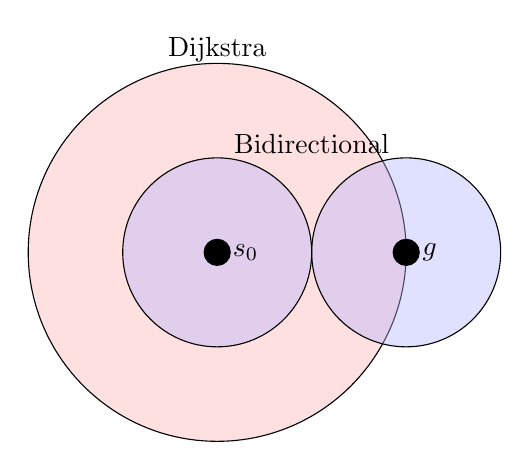
\begin{tikzpicture}[scale=0.6]
    \pgfmathsetmacro{\x}{2}
% forward search
\draw[fill=red!30, fill opacity=0.4] (0, 0) circle (2*\x);

% bidirectional search
\draw[fill=blue!30, fill opacity=0.4] (0, 0) circle (1*\x);
\draw[fill=blue!30, fill opacity=0.4] (2*\x, 0) circle (1*\x);


\node[draw,circle,fill=black] (a) at (0,0) {};
\node (aa) at (0+0.6, 0) {$s_0$};

\node[draw,circle,fill=black] (b) at (2*\x,0) {};
\node (bb) at (2*\x+0.5,0) {$g$};

\node (d) at (0, 2*\x+0.3) {Dijkstra};
\node (a) at (\x, 1*\x+0.3) {Bidirectional};

  \end{tikzpicture}
\end{figure}

\end{document}
